\VerdierPhysicalPageAnchor{0055}%
\VerdierSemanticAnchor{ch1-1-5-4-eq4}
D'après ce qui précède, nous savons que la propriété $P(\lambda,\mu)$
est vérifiée dans les cas suivants :

\begin{equation}
  \begin{gathered}
    \lambda\ \text{et}\ \mu\in\mathbb Z^{n-1},\\
    \lambda\ \text{et}\ \mu\in\mathbb Z e_n,\\
    \lambda\in\mathbb Z^{n-1}\ \text{et}\ \mu\in\mathbb Z e_n,\\
    \lambda\in\mathbb Z e_n\ \text{et}\ \mu\in\mathbb Z^{n-1}.
  \end{gathered}
  \tag{1.5.4.4}
\end{equation}

De plus (1.5.5), on a :

\VerdierSemanticAnchor{ch1-1-5-4-eq5}
\begin{quote}
  \noindent\textup{(1.5.4.5)}\quad
  \emph{Si trois des propriétés $P(\mu,\nu)$,
  $P(\lambda+\mu,\nu)$, $P(\lambda,\mu+\nu)$, $P(\lambda,\mu)$
  sont vraies, la quatrième l'est aussi.}
\end{quote}

\VerdierSemanticAnchor{ch1-1-5-4-conclusion}
On en déduit que la propriété $P(\lambda,\mu)$ est vraie pour tout
couple $\lambda,\mu\in\mathbb Z^n$, ce qui achève la démonstration de
la proposition (1.5.2).

\VerdierSemanticAnchor{ch1-1-5-5}
\noindent\textbf{Diagramme 1.5.5.}\quad
On se propose de démontrer l'assertion (1.5.4.5). On désigne par
$D(\lambda,\mu)$ le diagramme
$\textup{(1.5.4.1)}_{\lambda,\mu}$. La démonstration de (1.5.4.5)
repose sur la considération du diagramme que nous écrivons, pour
simplifier, dans le cas où les isomorphismes de transition $c$ et
$c'$ sont des morphismes identiques, \emph{i.e.} dans le cas où le
groupe $\mathbb Z^n$ opère strictement sur les catégories
$\mathcal C$ et $\mathcal C'$ :

\VerdierSemanticAnchor{ch1-1-5-5-tetrahedron}
\begin{center}
  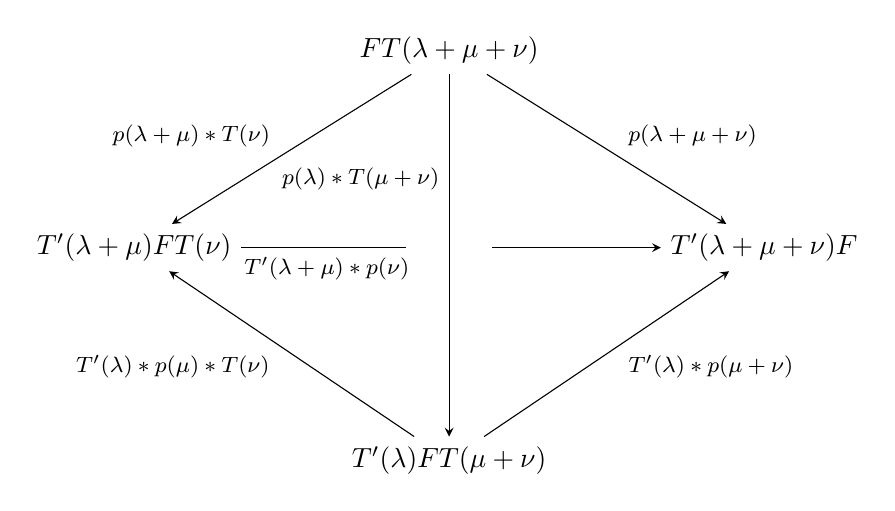
\begin{tikzpicture}[x=1cm,y=1cm,>=stealth]
    \node (a) at (0,3.2) {$FT(\lambda+\mu+\nu)$};
    \node (b) at (-4,0.7) {$T'(\lambda+\mu)FT(\nu)$};
    \node (c) at (4,0.7) {$T'(\lambda+\mu+\nu)F$};
    \node (d) at (0,-2.0) {$T'(\lambda)FT(\mu+\nu)$};
    \draw[->] (a) -- node[above left,pos=.55,font=\footnotesize]
      {$p(\lambda+\mu)*T(\nu)$} (b);
    \draw[->] (a) -- node[above right,pos=.55,font=\footnotesize]
      {$p(\lambda+\mu+\nu)$} (c);
    \draw[->] (a) -- node[left,pos=.29,font=\footnotesize]
      {$p(\lambda)*T(\mu+\nu)$} (d);
    \coordinate (bc-left) at (-0.55,0.7);
    \coordinate (bc-right) at (0.55,0.7);
    \draw (b) -- node[below,pos=.52,font=\footnotesize]
      {$T'(\lambda+\mu)*p(\nu)$} (bc-left);
    \draw[->] (bc-right) -- (c);
    \draw[->] (d) -- node[below left,pos=.55,font=\footnotesize]
      {$T'(\lambda)*p(\mu)*T(\nu)$} (b);
    \draw[->] (d) -- node[below right,pos=.55,font=\footnotesize]
      {$T'(\lambda)*p(\mu+\nu)$} (c);
  \end{tikzpicture}
\end{center}

\VerdierSemanticAnchor{ch1-1-5-5-faces}
Ce diagramme a la forme d'un tétraèdre dont les quatre faces sont
respectivement les diagrammes $D(\lambda,\mu+\nu)$,
$D(\lambda+\mu,\nu)$, $D(\lambda,\mu)T(\nu)$ et
$T'(\lambda)D(\mu,\nu)$. La démonstration de (1.5.4.5) se fait alors
en envisageant les quatre cas possibles et en utilisant la relation de
cocycle.

\VerdierSemanticAnchor{ch1-1-5-5-reduction}
Dans le cas général, le diagramme qu'il faut introduire est un peu
plus compliqué, mais en utilisant les identités (1.2.1.3), l'argument
se ramène à l'argument esquissé ci-dessus. Pour obtenir la démonstration
de (1.5.3.5), on utilise le même diagramme en posant :
\[
  \lambda=qe_1,\qquad \mu=q'e_1,\qquad \nu=q''e_1.
\]
